\section{Évaluation quantitative du modèle d'inventaire}\label{sec:meth_valid}
Comme il est mentionné dans la revue de littérature, la validation de modèles est une étape indispensable pour donner assez de confiance aux décideurs dans l'établissement de politiques publics. Cette section va donner un aperçu de la méthodologie utilisée en première approche et détailler une recommandation pour une validation plus complète. 

    \subsection{Sélection de lots pour la validation}
        Un échantillon de lots a été tiré au hasard pour faire la validation de l'inventaire. Puisqu'on essaie de qualifier le modèle par rapport à la réalité, les lots avec des données partielle ont été ignorés puisqu'on sait que les prédictions seront erronées pour ces lots. \par
        Un interface graphique a donc été créé pour permettre à l'utilisateur de créer l'ensemble de lots de validation et d'agréger des statistiques par catégorie. Ces catégories ont une définition récursive permettant à chaque strate d'avoir un ensemble de sous-catégories. Cette fonctionnalité peut être utile par exemple pour valider un segment de la population de lots de manière plus fine. L'interface permet de modifier les strates laissant de la flexibilité à l'utilisateur final. 
        \begin{table}[H]
            \centering
            \caption{Synthèse de sélection de lots de validation}
            \label{tab:sampling-strata-description}
            \begin{tabular}{m{3.25cm}                m{4.25cm}                          m{0.75cm}                    m{0.75cm}  m{0.75cm}m{1cm} m{1cm}  m{1cm}}
                \hline
                \multirow{2}{3.5cm}{Description}    & \multirow{2}{4cm}{Conditions} & \multirow{2}{0.75cm}{$n_{choisis}$}    & \multirow{2}{0.75cm}{$n_{obs}$}  & \multirow{2}{1cm}{$N$}    & \multicolumn{3}{c}{Données valides?} \\ 
                                                    &                               &                                       &                               &                           & Année & $N_{log}$ & Aire \\\hline
                Usage mixte                         & $N_{\text{CUBF}}>1$                  & 30                                    & 17                            & 156                       & Oui   & N/A       & Oui \\
                Usage unique                        & $N_{\text{CUBF}}=1$                  & N/A                                   & N/A                           & N/A                       & N/A   & N/A       & N/A \\
                \quad Résidentiel                   & $1000 \leq \text{CUBF}\leq 1999$     & N/A                                   & N/A                           & N/A                       & N/A   & N/A       & N/A \\
                \qquad Unifamilial                  & $N_{log}=1$                   & 30                                    & 30                            & 97748                     & Oui   & Oui       & N/A \\
                \qquad Plex                         & $ 2 \leq N_{log}\leq 8 $      & 30                                    & 30                            & 23621                     & Oui   & Oui       & N/A \\
                \qquad Appartements                 & $ 9 \leq N_{log}$             & 30                                    & 24                            & 2465                      & Oui   & Oui       & N/A \\
                \quad Industriel                    & $2000 \leq\text{CUBF}\leq 3999$     & 30                                    & 27                            & 176                       & Oui   & N/A       & Oui \\
                \quad Commerces                     & $5000 \leq \text{CUBF}\leq 5999$     & 30                                    & 30                            & 1552                      & Oui   & N/A       & Oui \\
                \quad Services                      & $6000 \leq \text{CUBF} \leq 6999$    & 30                                    & 27                            & 1623                      & Oui   & N/A       & Oui \\
                \quad Assemblée                     & $7000 \leq \text{CUBF} \leq 7999 $   & 30                                    & 23                            & 149                       & Oui   & N/A       & Oui \\ 
                Résidus                             &                               & 0                                     & 0                             & 13286                     & N/A   & N/A       & N/A\\ 
                \hline
                Total                           &                                    & 240                                  & 218                           & 140776                    &       &           & \\
            \end{tabular}
        \end{table}
        Tout cela étant dit, les études futures devraient utiliser la connaissance a priori de l'erreur de la méthode de prédiction pour modifier la structure des catégories pour aller chercher des détails sur des cas coins où l'on constate de fortes erreurs du modèle par rapport à la réalité pour mieux évaluer où et comment le modèle se comporte mal.\par
        
        
        Le tableau \ref{tab:sampling-strata-description} donne les paramètres des catégories d'évaluation choisie. Une allocation de 30 lots a été mise en place pour chaque catégorie. Les propriétés 
        

    
    \subsection{Méthode de quantification de l'erreur du modèle}
        Initialement, l'illustration d'une méthode d'équivalence paraissait souhaitable au début du processus d'évaluation de l'outil. Cependant, la compilation d'un effet minimum d'intérêt est ardue du fait d'un manque de cadre conceptuel d'utilisation. L'effet du stationnement sur les variables d'intérêt à différentes parties prenantes est à l'heure difficilement quantifiable du fait d'un manque de données de stationnement. \par
        Concernant la métrique d'intérêt, ce mémoire se concentrera sur l'erreur de prédiction par lot, mais compilera aussi les métriques traditionnelles comme l'erreur.\par
        De manière pratique, une approche par auto-amorçage a été choisie avec extraction des centiles avec 2000 répétitions a été implémentée pour l'erreur par lot. Pour le lot sélectionné, l'erreur entre la prédiction et l'observation est donnée par:
        \begin{equation}
            e_{h,i} = y_{h,i,o} - y_{h,i,p}
        \end{equation}
        où $e_{h,i}$ est l'erreur pour le lot $i$ de la catégorie $h$, $y_{h,i,o}$ est le nombre observé de places de stationnement,  $y_{h,i,p}$ est le nombre prédit de places soit $\lceil y_{h,i,min} \rceil$ le nombre de places minimums requises arrondies à l'entier supérieur. Les erreurs sont ensuite recentrées avant la procédure d'autoamorcage:
        \begin{equation}
            e_{h,c,i} = e_{h,i} - \frac{1}{n_h} \sum_{j=1}^{n_h} e_{h,j}
        \end{equation}
        Le vecteur d'erreur corrigées est ensuite constitué par l'équation suivante:
        \begin{equation}
            \mathbf{e}_{h,c} = \{e_{h,c,1},e_{h,c,2},\ldots, e_{h,c,n_h}\}
        \end{equation}
        La procédure d'autoamorçage est ensuite initiée avec ces erreurs centrées en réestimant l'erreur moyenne pour la catégorie. Un modèle de centiles est utilisé en première approche sans modèle de correction du biais ou de la variance. Cette approche est simpliste et la section \ref{sec:eval-park-pred-perf} montrera que certaines strates ont de fortes variations d'erreur avec le nombre de places prédites. D'autre part, ceci constitue un intervalle de prédiction de l'erreur moyenne. Il décrit quelle est l'erreur entre le modèle et une population semblable à celle tirée dans l'échantillon mais ne peut faire de prédiction sur la valeur réelle du stationnement. Il s'agit ici de la mesure d'un écart entre le modèle et un sous-ensemble de la population, pas une mesure de valeurs possibles de la variable d'intérêt (ici, le stationnement). Cette procédure est développée séparément de l'outil principal. Ceci est du à un manque de temps pour l'intégrer dans l'outil principal. Les scripts de validation peuvent être trouvés sur un dépôt Github supplémentaire\parencite{charbonneau_epmpaulpolyerror_propagation_2025}
    \subsection{Objets d'intérêt à la validation}
        \subsubsection{StrateEchantillon}
            Un objet est implémenté dans Typescript pour manipuler les catégories de validation. La description de strate est issue de la théorie d'échantillonnage, mais est évitée dans le cadre du mémoire pour éviter la confusion entre les méthodes inductives et la validation de modèle. Contrairement à la structure de données dans la base de données, l'objet utilise une structure de donnée récursive pour pouvoir créer un arbre pour les strates. Chaque entrée crée une seule condition sur une colonne de la table \ul{input\_validation}. Les paramètres de l'objet sont les suivants: 
            \begin{itemize}
                \item id\_strate: l'identifiant de la strate
                \item nom\_strate: une brève description
                \item nom\_colonne: la colonne de la table \ul{inputs\_validation} à laquelle s'applique la condtion
                \item ids\_enfants: une liste des id\_strate des strates qui sont sous cette strate dans l'arbre
                \item est\_racine: booléen indiquant que la strate est en haut de l'arbre (i.e cette strate est la première chargée dans la récursion) 
                \item index\_ordre: index pour permettre (à terme ) de changer l'ordre des strates dans la visualisation
                \item logements\_valides: condition supplémentaire pour indiquer que le nombre de logements doit être valide pour les entrées de cette strate
                \item date\_valide : condition supplémentaire pour indiquer que le nombre de logements doit être valide pour les entrées de cette strate
                \item superf\_valide : condition supplémentaire pour indiquer que la superficie to doit être valide pour les entrées de cette strate
                \item n\_sample: spécifie la taille d'échantillon pour la strate
                \item condition: une structure de donnée pour définir les conditions numériques qui s'applique sur la colonne spécifiée dans nom\_colonne 
                    \begin{itemize}
                        \item condition\_type: définit le type de condition comme une valeur unique (\og{equals}\fg{}) ou une étendue (\og{range}\fg{})
                        \item condition\_min: minimum de l'étendue si la condition est de type \og{range}\fg{}
                        \item condition\_max: maximum de l'étendue si la condition est de type \og{range}\fg{}
                        \item condition\_valeur: valeur que doit avoir la colonne si la condition est de type \og{equals}\fg{}
                    \end{itemize}
                \item substrata: les strates dont les identifiants sont sauvegardés dans ids\_enfants
            \end{itemize}
            L'implémentation actuelle est plus procédurale dans qu'orientée objet et mériterait d'être améliorée dans des versions futures de l'outil. 
    \subsection{Structure de données de l'échantillon de la validation}
        La validation requiert en elle-même une structure de données pour définir les strates, entreposer les résultats ainsi que d'entreposer des données ancillaires. La figure \ref{fig:erd-validation-stat} montre le diagramme entité relation pour entreposer les données de validation
        \begin{figure}[H]
            \centering
            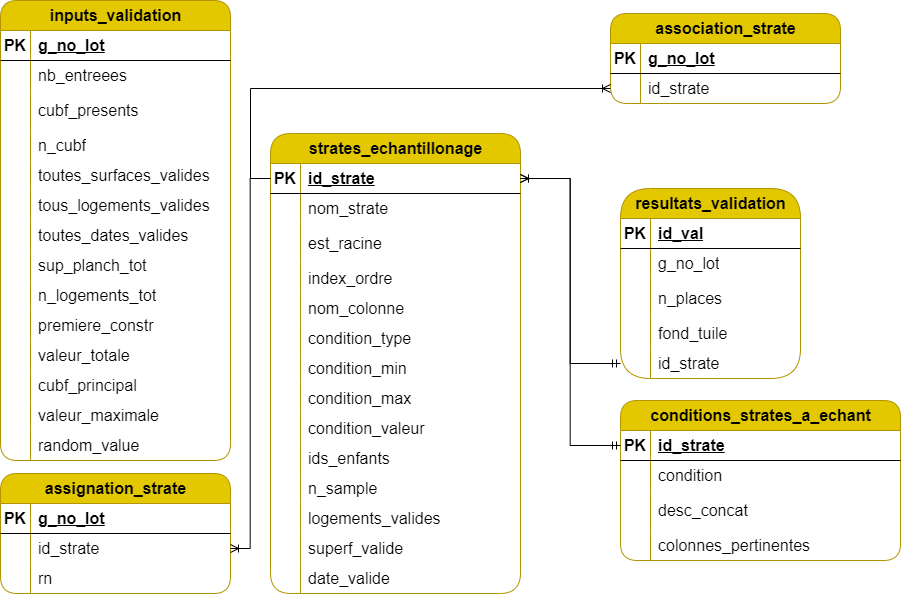
\includegraphics[width=0.8\linewidth]{images/ERD_stationnement_validation-2025-10-30.png}
            \caption{Diagramme entité relation pour la validation de l'inventaire}
            \label{fig:erd-validation-stat}
        \end{figure}
        \subsubsection{Définition des strates}
        La table \ul{strates\_echantillonage} contient la définition des paramètres des catégories de validation, reprenant la définition de l'objet mais sans les strates enfants et avec la condition aplatie dans la table. Le tableau \ref{tab:definition_strates} en donne la définition.
        \begin{longtable}{m{0.2\textwidth}|m{0.4\textwidth}m{0.2\textwidth}m{0.075\textwidth}}
                \caption{Colonnes pour la table \underline{strates\_echantillonage}}\label{tab:definition_strates}\\
                \hline
                Nom champ & Description & Type de données & CP/CS  \\
                \hline
                \endfirsthead
                \multicolumn{4}{c}%
                {{\tablename\ \thetable{} -- suite de la page précédente}} \\[0.5ex]
                \hline
                Nom champ & Description & Type de données & CP/CS  \\
                \hline
                \endhead
                \hline
                \endfoot
                
                id\_strate & Identifiant de la strate & Entier & CP \\
                nom\_strate & Description de la strate visible à l'usager & Texte & \\
                est\_racine & Booléen pour indique que la strate est un point d'entrée & Booléen & \\
                index\_ordre & Paramètre non-utilisé pour changer l'ordre d'affichage & Entier & \\
                nom\_colonne & Nom de la colonne à laquelle s'applique la condition & Texte & \\
                condition\_type & Type de condition & Texte \begin{compactitem} \item \og{range}\fg{} \item \og{equals}\fg{} \end{compactitem} & \\
                condition\_min & Minimum de l'étendue si condition\_type est range & Float & \\
                condition\_max & Maximum de l'étendue si condition\_type est range & Float & \\
                condition\_valeur & Valeur de la colonne si condition\_type est equals & Float & \\
                ids\_enfants & Identifiants des strates enfants & Liste d'entiers & \\
                n\_sample & Taile de l'échantillon & Entier & \\
                logements\_valides & Spécifie si les membre de la strate doivent avoir des valeurs de logements présentes sur toutes les entrées & Booléen \begin{compactitem} \item Vrai = doit être vrai \item Faux = doit être faux \item NULL = est ignoré \end{compactitem} & \\
                dates\_valides & Spécifie si les membres de la strate doivent avoir une date de construction valide sur toutes les entrées & Booléen \begin{compactitem} \item Vrai = doit être vrai \item Faux = doit être faux \item NULL = est ignoré \end{compactitem} & \\
                superf\_valide & Spécifie si les membres de la strate doivent avoir une superficie valide sur toutes les entrées & Booléen \begin{compactitem} \item Vrai = doit être vrai \item Faux = doit être faux \item NULL = est ignoré \end{compactitem} & \\

        \end{longtable}\clearpage
        \subsubsection{Données de lots pour la sélection} 
        Les données de lots pour la sélection sont agrégées dans la table \ul{inputs\_validation}. Les données sont compilées à l'aide de la requête présentée à l'annexe \ref{ann:intants-validation}. Les champs de la table sont données au tableau \ref{tab:definition_inputs_validation}
        \begin{longtable}{m{0.25\textwidth}|m{0.4\textwidth}m{0.1\textwidth}m{0.075\textwidth}}
            \caption{Colonnes pour la table \underline{inputs\_validation}}\label{tab:definition_inputs_validation}\\
            \hline
            Nom champ & Description & Type de données & CP/CS  \\
            \hline
            \endfirsthead
            \multicolumn{4}{c}%
            {{\tablename\ \thetable{} -- suite de la page précédente}} \\[0.5ex]
            \hline
            Nom champ & Description & Type de données & CP/CS  \\
            \hline
            \endhead
            \hline
            \endfoot
            g\_no\_lot & Identifiant de lot & Texte & CP \\
            nb\_entrees & Nombre d'entrées du rôle pour le lot & Entier & \\
            cubf\_presents & Liste des \ac{CUBF} uniques pour le lot & Entier & \\
            n\_cubf & Nombre de codes d'utilisation du bien fonds & Entier & \\
            toutes\_surfaces\_valides & Booléen indiquant que toutes les entrées du rôle ont l'aire d'étage entrée & Booléen & \\
            tous\_logements\_valides & Booléen indiquant que toutes les entrées du rôle ont un nombre de logements spécifiés & Booléen & \\
            toutes\_dates\_valides & Booléen indique que toutes les entrées du rôle ont des dates de construction entrées  & Booléen & \\
            sup\_planch\_tot & Superficie totale de plancher du lot & Float & \\
            n\_log\_tot & Nombre de logements total sur le lot & Entier & \\
            premiere\_constr & Première année de construction sur le lot & Entier & \\
            valeur\_totale & Valeur totale inscrite au rôle pour le lot & Entier & \\
            cubf\_principal & \ac{CUBF} de l'entrée du rôle avec la plus grande valeur & Entier & \\
            random\_value & Valeur pseudo-aléatoire affectée au lot & Réel & \\
        \end{longtable}
        \subsubsection{Association des lots aux strates et assignation à l'échantillon}     
        La table \ul{association\_strate} est principalement destinée à des fins de vérification de l'assignation aux strates. Elle contient seulement deux champs: id\_strate, l'identifiant de strate et g\_no\_lot l'identifiant de strate. \par
        La table \ul{assignation\_strate} contient les échantillons choisis pour la validations et contient n\_sample entrées pour chaque strate. Les champs sont les suivants: id\_strate, g\_no\_lot et rn, le rang du chiffre aléatoire assigné au lot. 
        \subsubsection{Résultats de validation}
        La table \ul{resultats\_validation} contient l'information pertinente au nombre de places comptées sur le lot, ainsi que le fond de tuile utilisé pour le compte qui est récolté quand l'usager enregistre l'entrée.
        \begin{table}[H]
            \caption{Colonnes pour la table \underline{resultats\_validation}}
            \label{tab:definition_resultats_valid}
            \centering
            \begin{tabular}{m{0.15\textwidth}|m{0.4\textwidth}m{0.2\textwidth}m{0.075\textwidth}}
                \hline
                Nom champ & Description & Type de données & CP/CS  \\
                \hline
                id\_val & Identifiant unique d'entrée & Entier & CP \\
                id\_strate & identifiant de strate & Entier & CS \\
                g\_no\_lot & Identifiant de lot & Texte & CS \\
                n\_places & Nombre de places comptées & Entier & \\
                fond\_tuile & Identifiant de fond de tuile lors de la sauvegarde  & Texte: \begin{compactitem}\item OSM \item Géodésie Québec \item ESRI \end{compactitem}  & \\
                \hline
           \end{tabular}
        \end{table}
        \FloatBarrier\clearpage
        \subsubsection{Propriétés agrégées de strate}
        La nature récursive de la structure de données de strates rend l'affichage de titres de strates ainsi que la vérification des conditions d'échantillonages potentiellement difficile. Cette table ne contient que les strates n'ayant pas d'enfants puisque ces dernières sont celles qui définissent vraiment l'échantillon. Le tableau \ref{tab:def-conditions-feuilles} donne les champs de cette table. Il est important de noter que les conditions listées ici sont typiquemetn utilisées à des fins de diagnostic. Les conditions sont toujours regénérées dans le serveur à partir de la définition dans la table \ul{strates\_echantillonage}
        \begin{table}[h]
            \caption{Colonnes pour la table \underline{conditions\_strates\_a\_echant}}
            \label{tab:def-conditions-feuilles}
            \centering
            \begin{tabular}{m{0.25\textwidth}|m{0.4\textwidth}m{0.15\textwidth}m{0.075\textwidth}}
                \hline
                Nom champ & Description & Type de données & CP/CS  \\
                \hline
                id\_strate & Identifiant unique de strate & Entier & CP \\
                condition & Condition en format SQL pour extraire les données & Texte & \\
                desc\_concat & Concaténation des noms des strates parents de la strate & Texte & \\
                colonnes\_pertinentes & Colonnes utilisées dans la requête & Liste de texte & \\
                \hline
           \end{tabular}
        \end{table}